\label{sec:intro}


%It also provides a rich source of information about the
%natural scene and hence 
Texture refers to a surface characteristic and appearance of an object given by
its geometry, density and surface reflectance, and the stochastic variation of
these parameters.
It is a detailed pattern that is mapped into a multidimensional space.
It is an important cue in trying to achieve photorealistic
rendering of 3D models by adding surface details or color to an object or a
scene. 

3D Texture modelling is an important area in computer graphics as it results in realistic rendering
of natural material surfaces.The characterization of surface reflectance properties is important in
achieving photorealism.The appearance of a surface in different lighting and viewing direction/
conditions is affected by its reflectance properties.3D texture actually models the relation
between surface reflectance properties and illumination direction.

%2D texture modelling fails to capture the surface variation and reflectance properties under
%varying lighting and viewing direction.They appear good only when viewed from similar lighting
%direction in which they were captured.2D textures appear flat and smooth but reflectance properties
%of real world objects are characterised by inter-reflections,shadows,specularity and sub-surface
%scattering. 2D texture fails to provide the information required for rendering other than the original
%illumination condition. Figure 1 illustrates how  the same texture behaves differently under different lighting conditions.

%$44It is clear from thefigure that 2D texture which has only the color information alone is not sufficient for a realisitic
% rendering of real world texture
%and therefore 3D texture is needed.
%For example, planar walls can have stone textures mapped onto them for a
%very convincing and realistic image of a three dimensional stone wall.
\begin{figure}[t]
\centering
\subfigure[]{
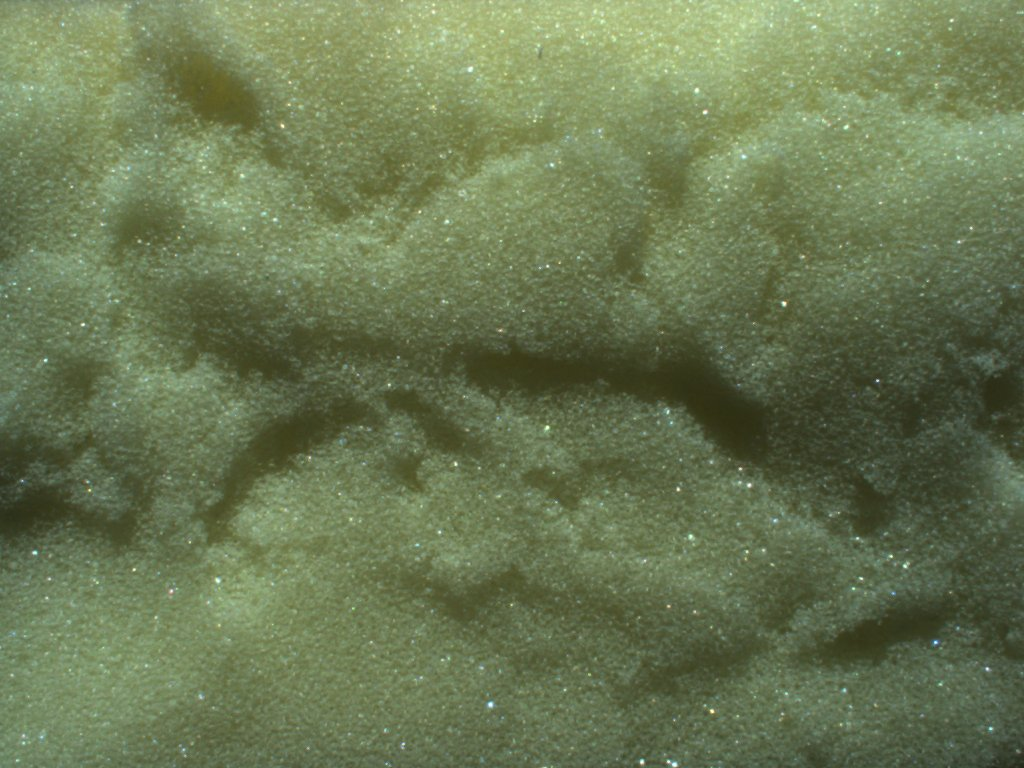
\includegraphics[scale=.15]{image_eps/orig_some/0.eps}
\label{fig:subfig1}
}
\subfigure[]{

\includegraphics[scale=.15]{image_eps/orig_some/9.eps}
\label{fig:subfig2}
}
\subfigure[]{
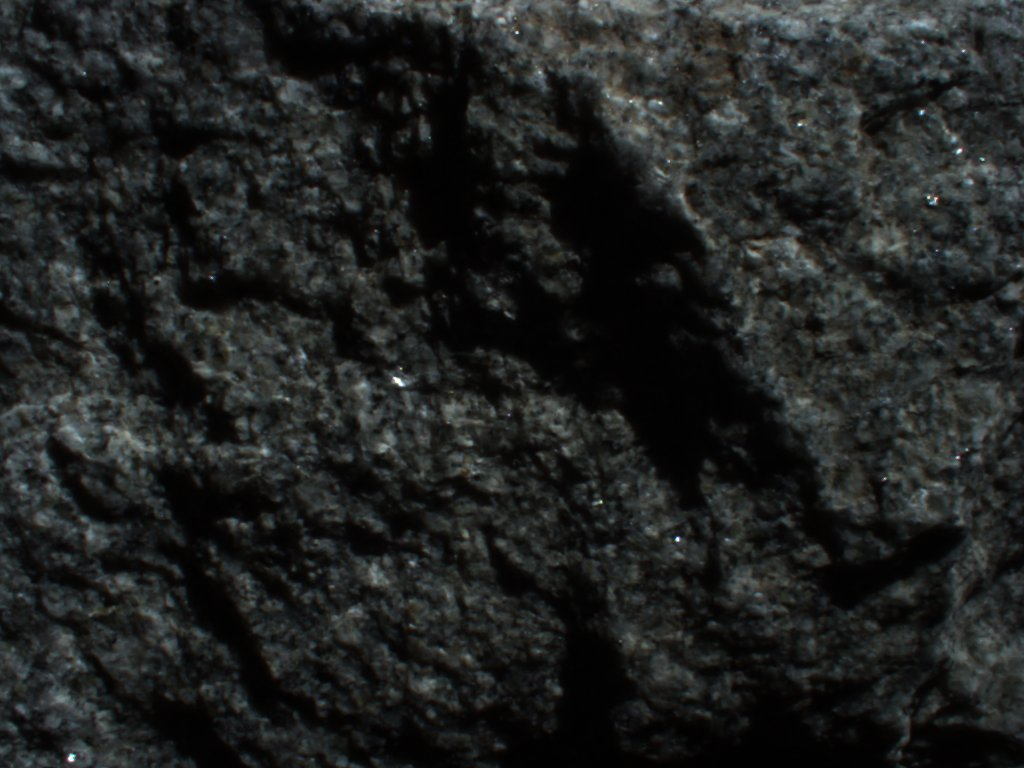
\includegraphics[scale=.15]{image_eps/orig_some/10.eps}
\label{fig:subfig3}
}
\subfigure[]{
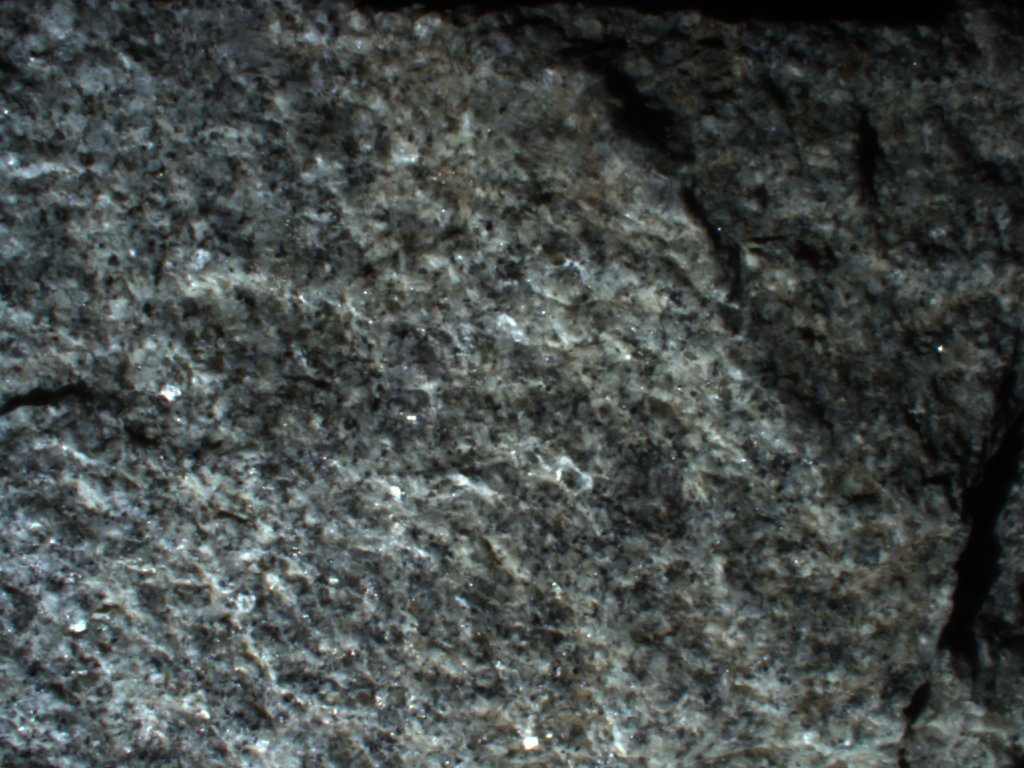
\includegraphics[scale=.15]{image_eps/orig_some/26.eps}
\label{fig:subfig3} }
\caption{Variation in appearance of the same surface
patch, when illuminated from different lighting directions.}
\label{fig:figure1}
\end{figure}
% However, the images mapped using this technique
%exhibit the properties of the lighting condition in which they were captured.
Mapping 2D textures or images is the most common method used, which is
efficient for most 3D models and scenes, especially where the lighting
conditions remain constant. They look best when the object is viewed in similar lighting conditions as
when the texture is captured. They appear flat and smooth.
In practice, the real world surfaces are
characterized by phenomena such as inter-reflection, self-shadowing, subsurface
scattering, specularity, etc. These properties interact with different lighting
directions and therefore the same surface appears different under
different lighting condition Fig.\ref{fig:figure1}. 2D texture fails to capture these complex reflectance properties of a 
surface and therefore a rendered surface looks highly unrealistic in case the lighting
conditions are changed. In order to produce a realistic rendering it is necessary to capture
and model the interaction of the material surface with different lighting
conditions. \cite{C1} investigates the problem of representation, recognition, synthesis of
natural materials and their rendering under arbitrary viewing/lighting conditions.

%They only model the reflectance properties of a surface,
%which alone is not sufficient for a realistic rendering of the real world
%materials. 



%%%%%%%%%%%%%%%%%FIGURE NO 1%%%%%%%%%%%%%%%

3D textures are a way to model this relation between surface reflectance
properties and illumination/viewing conditions.
The use of 3D texture modeling
results in enhanced realism of the scene. Reflectance texture maps are one of
the techniques that can be used to compactly represent the 3D textures. These
maps are generated using image re-lighting techniques \cite{C5,C4,C2} in which
multiple images are captured under different lighting conditions.

%Bidirectional Reflectance Distribution Function\cite{B1}, which defines the
%spectral and reflectance characteristics of a surface can be used to create
%reflectance texture maps. It is defined as the ratio of reflected radiance to
%incident irradiance, given the lighting and viewing directions. The reflectance
%at each point on a surface is hence a function of four parameters, controlling
%the above two directions. Various techniques have been developed to compactly
%represent BRDF \cite{B5,B8,B12,B14,B15}. It was extended to Bidirectional
%Texture Function \cite{B2} by allowing BRDF to vary spatially across planar
%texture co-ordinate (u,v).

%3D Texture modelling is an important area in computer graphics as it results in realistic rendering
%of natural material surfaces.The characterization of surface reflectance properties is important in
%achieving photorealism.The appearance of a surface in different lighting and viewing direction/
%conditions is affected by its reflectance properties.3D texture actually models the relation
%between surface reflectance properties and illumination direction. They are represented
%by Reflectance Texture Maps.These maps are generated using image re-lighting techniques
%\cite{B2,B6,B13} which model the surface reflectance properties of object.

%2D texture modelling fails to capture the surface variation and reflectance properties under
%varying lighting and viewing direction.They appear good only when viewed from similar lighting
%direction in which they were captured.2D textures appear flat and smooth but reflectance properties
%of real world objects are characterised by inter-reflections,shadows,specularity and sub-surface
%scattering. 2D texture fails to provide the information required for rendering other than the original
%illumination condition. Figure 1 illustrates how  the same texture behaves differently under different lighting conditions.

%It is clear from thefigure that 2D texture which has only the color information alone is not sufficient for a realisitic
% rendering of real world texture
%and therefore 3D texture is needed.

%Reflectance map required in 3D texture can be modelled by Bidirectional Reflectance Distribution
%Function \cite{B1} technique which defines spectral and spatial reflectance characteristic of a
%surface.BRDF is the ratio of reflected radiance to incident irradiance.Various techniques have been
%developed to compactly represent BRDF \cite{B5,B8,B12,B14,B15}.

%BRDF was extended to Bidirectional Texture Function \cite{B2} by allowing BRDF to vary spatially
%across planar texture co-ordinate (u,v)

%\begin{equation}
%BTF=(\theta_{v},\phi_{v},\theta_{e},\phi_{e},u,v)
%\end{equation}


%BTF effectively captures view point dependent phenomenon such as specularity
%along with other physical phenomenon such as shadow, sub-surface scattering,
%inter-reflection, etc. However, the capture of BTF requires careful camera
%calibration and capturing numerous images for sampling. Generating reflectance
%map from BTF is very complex. View dependent appearances can also be modeled
%using Light field maps \cite{B18}. They offer a more compact representation and
%can be used for a real time rendering of surface light fields.

%Because of the  high dimensionality of the BTF and high storage requirement,
%Unidirectional Texture Functions (UTF) were introduced in which viewing point is
%not taken into account while modeling the surface reflectance properties. They
%model these properties only in relation to different lighting conditions. As the
%visual appearance of the surface is mostly independent of the viewing direction,
%the model provides a reasonable approximation of the surface with significantly
%lower complexity of the model.

Image based modeling techniques \cite{C8,C6,C7} have emerged as
an effective approach for realistic rendering of 3D objects,
where multi-view geometry is utilized in directly synthesizing 
an unseen view of an object from nearby views without
explicit surface reconstruction. The traditional object models capture the shape information in the meshes,
while the reflectance and the surface properties are relegated in the textures. 3D models such as PTM capture the 
surface properties more faithfully, including the effect of small scale height variation on the surface.

Polynomial Texture Maps \cite{C4} belong to the class of UTFs (Uni-directional Texture Function). It is a pixel
based technique that concisely models the surface reflectance properties using a
polynomial model for the reflectance, dependent on two angular parameters of the
lighting direction ($l_u$ and $l_v$). It uses a
biquadratic polynomial function with 6 coefficients per pixel for modeling the
reflectance. PTMs reconstruct the color of the surface under varying
lighting conditions and models real world phenomenon such as
self-shadowing, inter-reflection and sub-surface scattering. They thus introduce
enhanced photorealism in texture mapping.
Polynomial Texture Mapping is applied in a wide
range of archaeological contexts \cite{C14}. 
It also offers advantages over traditional raking
light photography for examining and
documenting the surface texture and
shape of paintings \cite{C13}.
Recently, PTMs have been used in cultural heritage field to document and virtually inspect 
several sets of small objects, such as cuneiform tablets and coins.
%In the following section we
%summarize the results of our recent applications in conservation
%recording and comparison, analysis of archaeological materials,
%archaeological representation and dissemination.


%\subsection{3D texture VS 2D texture}

%In 2D texture modelling,the reflectance and the strutural properties of natural surfaces
%are not captured.They fail to capture the variations in surfaces for different lighting and
%viewing directions.In ed texture mapping the texture which is mapped onto a 3d model has
%the lighting direction from which it was captured.So if we want to see how the texture looks from
%different lighting direction,this mapping will give poor results when viewed from different
%lighting direction apart from the direction from which it was captured.In general,Real world objects
%are not flat and smooth in nature.They show different types of structural variation across their
%surface each having different reflectance properties.These properties causes effects like shadows,
%specularity sub-surface scattering,inter-reflection etc.Hence 3d texture mapping
%is required for realisting modelling of real objects.

%\subsection{BRDF}

%Reflectance texture maps are compact model for representing 3d textures.They model the spatial
%variation in surface luminance as a function of viewing and illumination direction.
%The bidirectional reflectance function \cite{A3} characterizes the color of a surface as a function
%of incident light and view directions.

%The BRDF is the ratio of the reflected intensity in the exitant direction to the incident
%energy per unit area along the incident direction.

%\subsection{PTM}
%Polynomial Texture Maps \cite{A1} is a pixel based technique used to model luminiance
%against changing lighting direction.PTMs reconstruct the color of a surface under varying lighting
%conditions. When a surface is rendered with a PTM, it takes on different illumination
%characteristics depending on the direction of the light source.

%PTM model uses a set of input images captured from a fixed camera, where each
%image is illuminated from a specific known lighting direction. It uses a
%biquadratic polynomial function with 6 coefficients per pixel for modeling the
%reflectance. These coefficients are estimated from the set of input images(30 to
%40), where the lighting direction is resolved into two components i.e
%$l_{u}$,$l_{v}$ by projecting it on the image plane. These two components are
%used as variables in the biquadratic function. Once the coefficients are
%estimated fitting the model to the observed values, they are used to render
%images from any given lighting direction.


In this thesis, 
we propose an approach to image-based lighting interpolation that is
based on estimates of geometry and shading from a set of input images.
\section{Problem}

PTM technique causes overall smoothening of light which dampens the effect
of specularity and softens sharp shadows. The effect of point light source is
reduced and the appearance is always similar to a diffused light source.
We improve upon the PTM model 
to overcome the above limitations
and generate a complete 3D Texture model that can be evaluated at individual
pixels.  
%The current state-of-the art
%in the field of PTM involves robust method for interpolation of shadow and specularity,Drew {\em et al.}\cite{A10} 
%But they do not model natural material surfaces and their interactions
%with changing light conditions.
%Moreover the number of per pixel parameters are too high for real-time rendering. 
%\cite{A3} shows that surface normals
%extracted from the PTM image data structure are of lower
%quality because of the smoothing caused by the use of biquadratic function, which compromises the directional 
%accuracy of the normals.
%PTM. The directional accuracy of the normals is compromised
%by the PTM biquadratic function’s smoothing over the range of
%illumination angles in the hemisphere
\section{Motivation}
Texture mapping is an important area in computer graphics which adds realism to three dimensional models.
2D texture mapping fails to capture the surface variation and reflectance properties under
varying lighting and viewing direction. They appear good only when viewed from similar lighting
direction in which they were captured and fails to provide the information required for rendering other than the original
illumination condition. But 3D textures correctly models the relation between surface reflectance
properties and illumination conditions.The use of 3D texture modeling
results in enhanced realism of the scene.

\begin{figure*}[t]
\centering
%\subfigure[]{
\includegraphics[height=3.4in,width=6.0in]{sep_images/sep3.eps}
%\label{fig:subfig23} } \caption[] {Components of a sponge image: a) Original image, b) Direct c) Global
%component.} 
\label{fig:2}
\caption{Component Based Modeling (CBM)}
\end{figure*}
\section{Approach}
We capture multiple images of a static object with a static camera under varying
lighting conditions.
The scene is
illuminated using a high frequency checkerboard pattern using the projector. The
projector is moved to different lighting positions for the purpose of obtaining
images with different lighting directions. Experimental setup is shown in Figure \ref{fig:figure3}

When we separate the image of the texture into direct and the global part, we find
that the shadows and the specularities appear very strongly in the direct part,
as these are phenomena that involve light that reaches the surface point
directly from the light source. The fine details and the structure of the
material are very prominently visible in the direct part as they are observed
primarily through shadows. On changing the lighting direction, the change in the
luminance of the direct part is minimal as long as the surface point is directly
illuminated. The variations are introduced, primarily by self-shadowing and
specularity, both of which are abrupt changes as the lighting direction changes.
The global component contains the the lighting of a surface point from other
parts in a scene, and hence the captures the overall illumination as well as
color variations of a surface with lighting direction. As the lighting direction
changes, the luminance value of the global part varies significantly.

Both direct and global components are separately analyzed to derive the
corresponding models and parameters. Given a new lighting direction, we use the
two models separately to generate the corresponding components, and combine them
to get the final image.Then for a new lighting direction, we can readily
interpolate both specular content as well as shadows.
% We decompose images captured at different lighting conditions into intrinsic image
% components; i.e, the {\em direct} and {\em global} image components. Each of
% these components is then further separated to obtain different physical
% phenomena such as shadows, specularity and luminance. The final image is obtained
% by combining the individual models together.
The method is shown to indeed
generate better results for non-observed lighting directions.
\begin{figure}[t]
\centering
\subfigure{
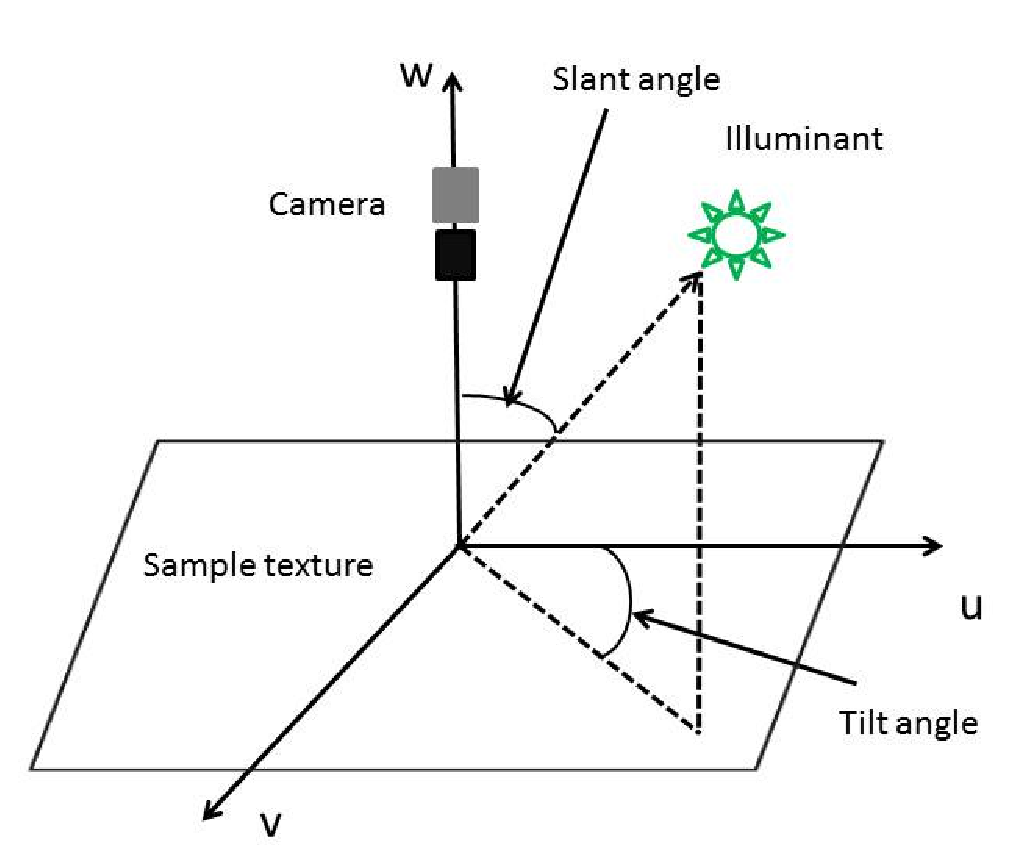
\includegraphics[scale=.56]{chap3/res_2/setup.eps}
\label{fig:figure3}
}
\caption{Experimental setup}
\end{figure}
\section{Contribution}
The main contributions are (1) Direct and Global modeling characterized by
shadows,specularity and luminance, 
(2) separate modeling and hence better capturing of shadows and specularities 
and (3) per pixel function model to
achieve real-time rendering of enhanced 3D textures on GPU.

\section{Outline}
The rest of this thesis is organized as follows: We will survey techniques 
related to texture mapping in Chapter 2. In Chapter 3
component based modeling will be discussed where we will show how each component is
modeled differently. 
we will explain
shadow and specularity modeling
In Chapter 4, we apply our model for extracting text 
inscribed in walls. Finally we 
conclude the thesis and discuss future work in Chapter 5.

% Texture mapping adds realism details to raster images with relatively small increase in
% computation and has long been used in computer graphics. Texture can be defined in the
% usual sense (such as cloth, wood, brick and so on), more specifically a detailed pattern or a
% multidimensional image that is mapped into a multidimensional space. In the latter form,
% a photograph is used to map onto a planar surface, which avoids modeling complex surface
% details. However this method fails when the lighting conditions of the synthetic environment
% are different from those of the texture image and the results will look unrealistic and flat [17].
% Due to these problems, the field of image based modeling and rendering (IBMR) has
% attracted people's attention in recent decades. IBMR methods rely on a set of two dimen-
% sional images as inputs. In order to obtain photorealistic rendering, one should be able to
% characterize surface reflectance properties such as surface normal and albedo.

% Texture refers to a surface characteristic and appearance of an object given by
% its geometry, density and surface reflectance, and the stochastic variation of
% these parameters. It also provides a rich source of information about the
% natural scene and hence is important cue in trying to achieve photo realistic
% rendering of 3D models by adding surface details or color to an object or a
% scene. For example, planar walls can have stone textures mapped onto them for a
% very convincing and realistic image of a three dimensional stone wall.

% Mapping 2D textures or images is the most common method used, which is both
% efficient effective for most 3D models and scenes, especially where the lighting
% condition remain constant. However, the images mapped using this technique
% exhibit the properties of the lighting condition in which they were captured.
% Hence they look best when the object is viewed in similar lighting conditions as
% when the texture is captured. In practice, the real world surfaces are
% characterized by phenomena such as inter-reflection, self-shadowing, subsurface
% scattering, specularity, etc. These properties interact with different lighting
% directions conditions and therefore the same surface appears different under
% different lighting condition(see Figure 1).
% 
% 2D texture fails to capture these complex reflectance properties of a surface
% and therefore a rendered surface looks highly unrealistic in case the lighting
% conditions are changed. They only model the reflectance properties of a surface,
% which alone is not sufficient for a realistic rendering of the real world
% materials. In order to produce a realistic rendering it is necessary to capture
% and model the interaction of the material surface with different lighting
% conditions.


%%%%%%%%%%%%%%%%%FIGURE NO 1%%%%%%%%%%%%%%%





%----------------------------------------------------------------------
%\section{First Section} 
%\label{sec:SECTION1NAME}

%Text of section 1 goes here... \\

%This is to insert a table \\

%\begin{table}
%\begin{center}
%\begin{tabular}{|l|c|}
%\hline
%Method & Frobnability \\
%\hline\hline
%Theirs & Frumpy \\
%Yours & Frobbly \\
%Ours & Makes one's heart Frob\\
%\hline
%\end{tabular}
%\end{center}
%\caption{Results.   Ours is better.}
%\end{table}

%This is to insert a figure \\

%\begin{figure}[h]
%\centering
%
\includegraphics[height=2cm,width=0.2\linewidth]{figures/iiit.eps}
%\caption{Analysis of our method}
%\label{}
%\end{figure}



%----------------------------------------------------------------------
%\section{Second Section} 
%\label{sec:SECTION2NAME}

%Text of section 2 goes here... \\

%{\bf Few suggestions}

%-------------------------------
%\subsection{Mathematics}

%Please number all of your sections and displayed equations.  It is
%important for readers to be able to refer to any particular equation.  Just
%because you didn't refer to it in the text doesn't mean some future reader
%might not need to refer to it.  It is cumbersome to have to use
%circumlocutions like ``the equation second from the top of page 3 column
%1''.  (Note that the ruler will not be present in the final copy, so is not
%an alternative to equation numbers).  All authors will benefit from reading
%Mermin's description of how to write mathematics (see math.pdf).


%------------------------------
%\subsection{Footnotes}

%Please use footnotes\footnote {This is what a footnote looks like.  It
%often distracts the reader from the main flow of the argument.} sparingly.
%Indeed, try to avoid footnotes altogether and include necessary peripheral
%observations in 
%the text (within parentheses, if you prefer, as in this sentence).  If you
%wish to use a footnote, place it at the bottom of the column on the page on
%which it is referenced. Use Times 8-point type, single-spaced.

%--------------------------------
%\subsection{References}

%List and number all bibliographical references in 9-point Times,
%